\chapter{Architekturdiagramm}

\begin{comment}
Im Architekturdiagramm muss ersichtlich sein welche Softwareschichten/Softwarekomponenten es im System gibt und über welche Kommunikationsprinzipen und Protokolle diese miteinander kommunizieren. Es muss aufgezeigt werden wie die ausgetauschten Informationen repräsentiert werden. Des Weiteren spielt die Verteiltheit der Anwendungslogik eine große Rolle. 

Es muss nachvollziehbar sein inwiefern eine Verteiltheit der Anwendungslogik gegeben ist. 

Sämtliche Entscheidungen müssen begründet und abgewogen werden. Formal gesehen sollten einfache geometrische Primitive verwenden werden. (Orientierung an der Fachliteratur) 
\end{comment}



\section{Variante 1: API orientiert}

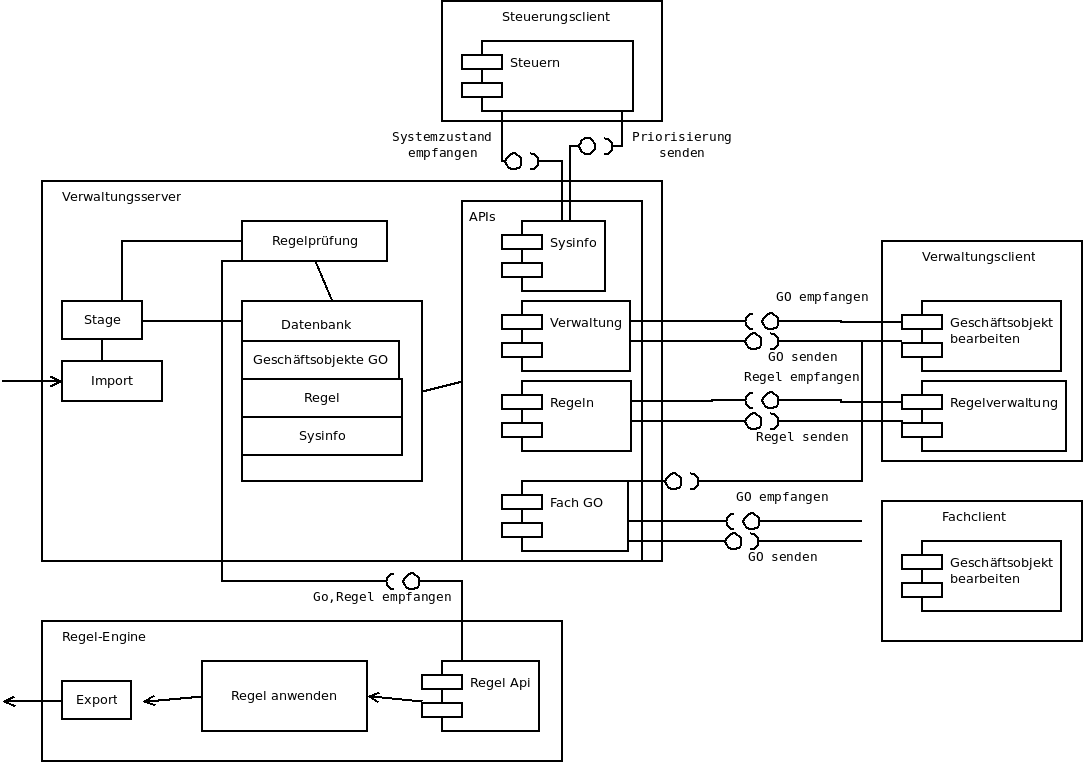
\includegraphics[width=\textwidth]{EISWS1516Howe_MS2_Architektur_api.png}

\pa

\section{Variante 2: Nachrichten orientiert}



\begin{comment}

\section{Übersicht}
- bsp arch\\
- arch mit ASys\\
- 

\section{Verwaltungsdienst}

\section{Clients}

\subsection{Verwaltung}
\subsection{Fachclient}

\section{Steuerungsclient}


\section{Regel-Engine}

\end{comment}


